\begin{figure}
  \centering
  \begin{tikzpicture}
    \draw[very thick,->] (0,0) -- (3.8,0) node[anchor=north] {x};
    \draw[very thick,->] (0,0) -- (0,3.3) node[anchor=east] {y};
    \node at (-0.2,0) {0};
    \node at (0,-0.2) {0};
    % final system
    \draw[dark-green, local bounding box=new, very thick]
      (0.7, 0.2) rectangle (4.2, 2.7);
    \draw[dark-green, dashed, very thick]
      ({$(new.west)$} |- {$(new.north)$}) --
      ({$(new.east)$} |- {$(new.south)$});
    \draw[dark-green, dashed, very thick]
      ({$(new.west)$} |- {$(new.south)$}) --
      ({$(new.east)$} |- {$(new.north)$});
    % first system
    \draw[red, local bounding box=S1, dashed, thick]
      (1.2,0.2) rectangle (3.7,2.7);
    \draw[red, dashed]
      ({$(S1.west)$} |- {$(S1.north)$}) --
      ({$(S1.east)$} |- {$(S1.south)$});
    \draw[red, dashed]
      ({$(S1.west)$} |- {$(S1.south)$}) --
      ({$(S1.east)$} |- {$(S1.north)$});
    % second system
    \draw[blue, local bounding box=S2, dashed, thick]
      (0.2,1.2) rectangle (3.2,3.2);
    \draw[blue, dashed]
      ({$(S2.west)$} |- {$(S2.north)$}) --
      ({$(S2.east)$} |- {$(S2.south)$});
    \draw[blue, dashed]
      ({$(S2.west)$} |- {$(S2.south)$}) --
      ({$(S2.east)$} |- {$(S2.north)$});
    \draw[blue, -latex]
      ({$(S2.west)!0.5!(S2.east)$} |- {$(S2.north)!0.5!(S2.south)$}) --
      ({$(new.west)!0.5!(new.east)$} |- {$(new.north)!0.5!(new.south)$});
    \node[dark-green]
      at ({$(new.west)!0.3!(new.east)$} |- {$(new.south)!1.10!(new.north)$})
      {New System};
  \end{tikzpicture}
  \hspace{30pt}
  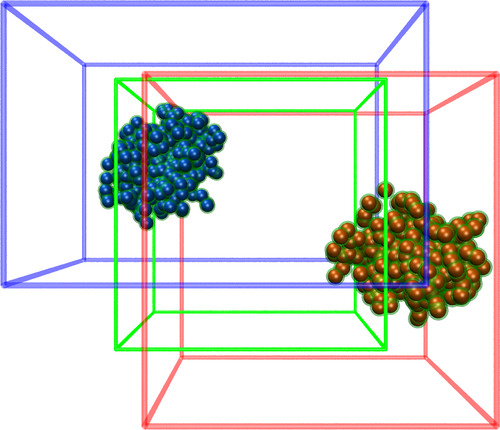
\includegraphics[scale=0.6]{JoinSystems-fig_c.jpg}
  \caption{
    Option \tt{-offset c c c} transposes the geometric centre of the second box
    (blue) on the centre of the first box (red), moving all beads from the
    second system with it.
  }
\end{figure}
